% % % % % % % % % % % % %
	% %inizio package view% %
	% % % % % % % % % % % % %
	\pagebreak
	\subsection{Romeo::View}
	\label{romeo::view}
		\subsubsection{Informazioni sul package}
		\label{view_info}
		\begin{figure}[!h]
			\centering
			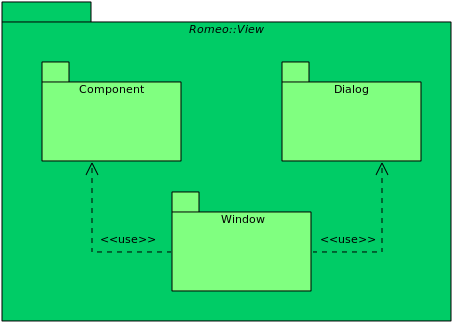
\includegraphics[width=\linewidth]{./Content/Immagini/Romeo__View.png}
			\caption{Componente Romeo::View}
			\label{comp_romeo::view}
		\end{figure}
		\subsubsection{Descrizione}
		\label{view_descr}
		Package\glossario{} che rappresenta la componente View dell'architettura MVC\glossario{}.
		\subsubsection{Package contenuti}
		\label{view_package}
		\begin{itemize}
			\item \hyperref[romeo::view::window]{Romeo::View::Window};
			\item \hyperref[romeo::view::dialog]{Romeo::View::Dialog};
			\item \hyperref[romeo::view::component]{Romeo::View::Component}.
		\end{itemize}		
		\subsubsection{Relazioni tra i componenti}	
		Il package\g{} Window utilizzerà vari componenti del package\g{} Component e del package\g{} Dialog per generare le varie finestre e dialoghi. Il diagramma seguente illustra le relazioni interne a Romeo::View tra le classi contenute nei vari package\g{}.
		\begin{figure}[!h]
			\centering
			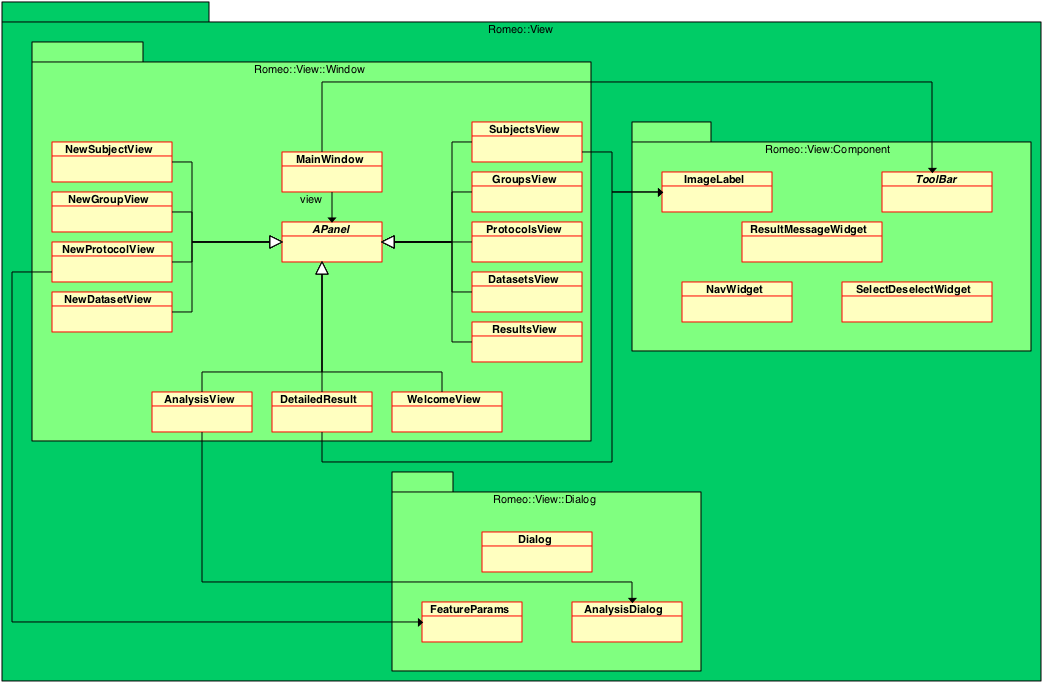
\includegraphics[width=1.1\linewidth]{./Content/Immagini/RelazioniView.png}
			\caption{Relazioni tra le classi del package Romeo::View}
			\label{Relview}
		\end{figure}
	\linebreak
	\pagebreak
	
		
	\subsection{Romeo::View::Window}
	\label{romeo::view::window}
		\subsubsection{Informazioni sul package}
		\label{info_window}
		\begin{figure}[!h]
					\centering
					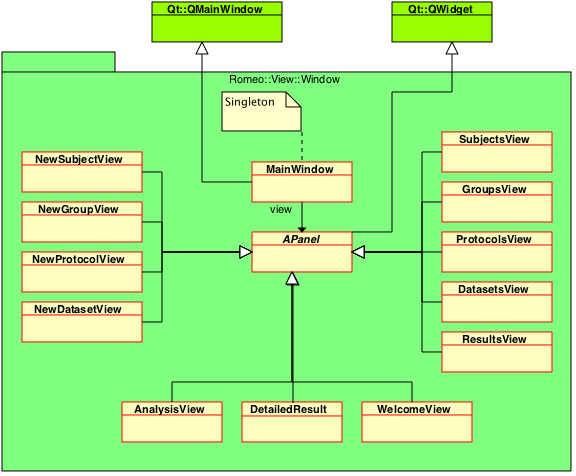
\includegraphics[width=\linewidth]{./Content/Immagini/Window.png}
					\caption{Diagramma package \textsl{Romeo::View::Window}}
					\label{comp_romeo::view::window}
				\end{figure}
		\subsubsection{Descrizione}
		\label{descr_window}
		Package\glossario{} che contiene l'insieme delle \lq\lq{}finestre\rq\rq{} con le quali l'utente può interagire durante l'esecuzione di \project{}.
		
		\subsubsection{Relazioni tra i componenti}
		La classe MainWindow contiene un riferimento polimorfo alla classe , classe astratta che rappresenta una generica finestra del programma.
		
		\subsubsection{Classi contenute}
			\paragraph{\underline{MainWindow}}
			\label{mainview}
				\subparagraph{Descrizione:} classe che rappresenta la finestra principale dell'applicativo \project{} con la quale l'utente interagisce.
				 Viene creata \emph{unicamente} al primo avvio del programma e rimane attiva fino alla chiusura del programma.
				\\È implementata tramite il design pattern\g{} Singleton.
				\subparagraph{Eredita da:}
					\begin{itemize}
					\item Qt::QMainWindow.
					\end{itemize}
				\subparagraph{Relazioni con altre classi:}
					\begin{itemize}
						\item \hyperref[ab_panel]{Romeo::View::Window::APanel}: relazione uscente, riferimento all'oggetto APanel che la MainWindow sta attualmente rappresentando;
						\item \hyperref[mbc]{Romeo::View::Component::MenuBar:} relazione uscente, riferimento al menù con il quale interagisce l'utente;
						\item \hyperref[tb]{Romeo::View::Component::ToolBar:} relazione uscente, riferimento alla toolbar con la quale interagisce l'utente;
						\item \hyperref[controller_main]{Romeo::Controller::MainWindowController}: relazione entrante, riferimento alla MainWindow che il controller sta \lq\lq{}controllando\rq\rq{}.
					\end{itemize}
			
		\paragraph{\underline{APanel}}
		\label{ab_panel}
			\subparagraph{Descrizione:} classe astratta che rappresenta un generico \lq\lq{}widget\rq\rq{} utilizzato dalla \hyperref[mainview]{MainWindow} come contenuto centrale. In un dato istante la \hyperref[mainview]{MainWindow} avrà sempre un \emph{unico} widget. Essendo una classe astratta non verrà mai utilizzata direttamente, ma verrà estesa dalle classi che verranno utilizzate nella MainWindow.
			\subparagraph{Eredita da:}
				\begin{itemize}
				\item Qt::QWidget.
				\end{itemize}
				
			\subparagraph{Ereditata da:}
			\begin{itemize}
				\item \hyperref[nsv]{Romeo::View::Window::NewSubjectView};
				\item \hyperref[ngv]{Romeo::View::Window::NewGroupView};
				\item \hyperref[npv]{Romeo::View::Window::NewProtocolView};
				\item \hyperref[ndv]{Romeo::View::Window::NewDatasetView};
				\item \hyperref[sav]{Romeo::View::Window::AnalysisView};
				\item \hyperref[drv]{Romeo::View::Window::DetailedResult};
				\item \hyperref[wv]{Romeo::View::Window::WelcomeView};
				\item \hyperref[vsv]{Romeo::View::Window::SubjectsView};
				\item \hyperref[vgv]{Romeo::View::Window::GroupsView};
				\item \hyperref[vpv]{Romeo::View::Window::ProtocolsView};
				\item \hyperref[vdv]{Romeo::View::Window::DatasetsView};
				\item \hyperref[vrv]{Romeo::View::Window::ResultsView}.
			\end{itemize}
			\subparagraph{Relazioni con altre classi:}
				\begin{itemize}
					\item  \hyperref[controller_a]{Romeo::Controller::AController}: relazione entrante, riferimento alla generica \lq\lq{}view\rq\rq{} che il controller sta \lq\lq{}controllando\rq\rq{}.
				\end{itemize}
		
		
		\paragraph{\underline{WelcomeView}}
		\label{wv} 
			\subparagraph{Descrizione:} classe che rappresenta la view iniziale del sistema. Permette all'utente di scegliere una tra le varie funzionalità del programma. 
			Viene creata all'avvio del programma e permette all'utente di selezionare una delle funzionalità presenti.
			\\Inoltre viene creata quando da una delle view l'utente decide di ritornare alla WelcomeView.
			Emette un signal\g{} in seguito alla scelta effettuata.
			\subparagraph{Eredita da:} 
				\begin{itemize}
					\item \hyperref[ab_panel]{Romeo::View::Window::APanel}.
				\end{itemize}
			\subparagraph{Relazioni con altre classi:}
				\begin{itemize}
					\item \hyperref[controller_wp]{Romeo::Controller::WelcomeController}: relazione entrante, tipo dinamico del riferimento posseduto del Controller. 
				\end{itemize}
				
		\paragraph{\underline{NewSubjectView}}
		\label{nsv}
			\subparagraph{Descrizione:} permette la creazione di un nuovo Subject\glossario{}. Viene creata ogni qualvolta l'utente seleziona, dalla WelcomeView, la funzionalità di creazione di un nuovo Subject\glossario{}. Emette un signal\g{} in seguito alla conferma, da parte dell'utente, della creazione di un nuovo Subject\glossario{}.
			\subparagraph{Eredita da:}
				\begin{itemize}	
					 \item \hyperref[ab_panel]{Romeo::View::Window::APanel}.
				\end{itemize}
			\subparagraph{Relazione con altre classi:}
				\begin{itemize}
					\item \hyperref[controller_ns]{Romeo::Controller::NewSubjectController}: relazione entrante, tipo dinamico del riferimento posseduto dal Controller.
				\end{itemize}
	
		\paragraph{\underline{NewGroupView}}
		\label{ngv} 
			\subparagraph{Descrizione:} permette la creazione di un nuovo gruppo di Subject\glossario{}. Viene creata ogni qualvolta l'utente seleziona, dalla WelcomeView, la funzionalità di creazione di un nuovo gruppo di Subject\glossario{}. Per essere creata necessita che almeno un Subject\g{} sia presente nel sistema.
			\\Inoltre permette la modificha di un gruppo di subject\g{} preesistente.
			 Emette un signal\g{} in seguito alla conferma, da parte dell'utente, della creazione di un nuovo gruppo di Subject\glossario{}.
			\subparagraph{Eredita da:}
				\begin{itemize}
					\item \hyperref[ab_panel]{Romeo::View::Window::APanel}.
				\end{itemize}
			\subparagraph{Relazione con altre classi:}
				\begin{itemize}
					\item \hyperref[controller_ngs]{Romeo::Controller::NewGroupController}: relazione entrante, tipo dinamico del riferimento posseduto dal Controller;
					\item \hyperref[controller_tm]{Romeo::Model::QtModel::NewGroupTableModel}: relazione uscente, riferimento al model della tabella visualizzata nella view.
				\end{itemize}
		
		\paragraph{\underline{NewProtocolView}}
		\label{npv} 
			\subparagraph{Descrizione:} permette la creazione di un nuovo Protocol\glossario{}. Viene creata ogni qualvolta l'utente seleziona, dalla WelcomeView, la funzionalità di creazione di un nuovo Protocol\glossario{}. Emette un signal\g{} in seguito alla conferma, da parte dell'utente, della creazione di un nuovo Protocol\glossario{}.
			\subparagraph{Eredita da:}
				\begin{itemize}
				 	\item \hyperref[ab_panel]{Romeo::View::Window::APanel}.
				\end{itemize}
			\subparagraph{Relazioni con altre classi:}
				\begin{itemize}
					\item \hyperref[controller_np]{Romeo::Controller::NewProtocolController}: relazione entrante, tipo dinamico del riferimento posseduto dal Controller;
					\item \hyperref[controller_tm]{Romeo::Model::QtModel::NewProtocolFeatureTableModel}: relazione uscente, riferimento al model della tabella visualizzata nella view.
				\end{itemize}
		 
	\paragraph{\underline{NewDatasetView}}
	\label{ndv}
		\subparagraph{Descrizione:} permette la creazione di un nuovo Dataset\glossario{}.
		viene creata ogni qualvolta l'utente seleziona, dalla WelcomeView, la funzionalità di creazione di un nuovo Dataset\glossario{}. Per essere creata necessita che almeno un gruppo di Subject\g{} e un Protocol\g{}, siano presenti nel sistema. Emette un signal\g{} in seguito alla conferma, da parte dell'utente, della creazione di un nuovo gruppo di Dataset\glossario{}.
		\subparagraph{Eredita da:}
			\begin{itemize}
			\item \hyperref[ab_panel]{Romeo::View::Window::APanel}.
			\end{itemize}
		\subparagraph{Relazioni con altre classi:}
			\begin{itemize}
				\item \hyperref[controller_nd]{Romeo::Controller::NewDatasetController}: relazione entrante, tipo dinamico del riferimento posseduto dal Controller;
				\item \hyperref[controller_tm]{Romeo::Model::QtModel::DatasetGroupTableModel}: relazione uscente, riferimento al model della tabella presente nella view che visualizza i Dataset;
				\item \hyperref[controller_tm]{Romeo::Model::QtModel::DatasetProtocolTableModel}: relazione uscente, riferimento al model della tabella presente nella view che visualizza i Protocol.
			\end{itemize}
	
	\paragraph{\underline{SubjectsView}}
	\label{vsv} 
		\subparagraph{Descrizone:} permette la visualizzazione dei Subject\glossario{} memorizzati nel sistema. Viene creata ogni qualvolta l'utente seleziona, dalla WelcomeView, l'opzione di visualizzazione della lista dei Subject\glossario{}. Essa comunica con il Controller per acquisire la lista dei Subject\glossario{}.
		\subparagraph{Eredita da:}
			\begin{itemize}
				\item \hyperref[ab_panel]{Romeo::View::Window::APanel}.
			\end{itemize}	
		\subparagraph{Relazioni con altre classi:}
			\begin{itemize}
				\item \hyperref[controller_ss]{Romeo::Controller::SubjectsController}: relazione entrante, tipo dinamico del riferimento posseduto dal Controller;
				\item \hyperref[controller_tm]{Romeo::Model::QtModel::SubjectTableModel}: relazione uscente, riferimento al model della tabella visualizzata nella view.
			\end{itemize}
		
	\paragraph{\underline{GroupsView}}
	\label{vgv} 
		\subparagraph{Descrizione:}
		classe che rappresenta la view per la visualizzazione, l'eliminazione e la modifica dei vari gruppi di Subject\glossario{} presenti nel sistema. Viene creata ogni qualvolta l'utente seleziona, dalla WelcomeView, l'opzione di visualizzazione dei lista dei gruppi di Subject\glossario{}. Comunica con il relativo controller per ottenere la lista dei gruppi di Subject\glossario{}, modificare un gruppo (aggiungendo o togliendo Subject\g{}) e per eliminare eventuali gruppi selezionati.
		\subparagraph{Eredita da:} 
			\begin{itemize}
				\item \hyperref[ab_panel]{Romeo::View::Window::APanel}.
			\end{itemize}
		\subparagraph{Relazioni con altre classi:}
			\begin{itemize}
				\item \hyperref[controller_sg]{Romeo::Controller::GroupsController}: relazione entrante, tipo dinamico del riferimento posseduto dal Controller;
				\item \hyperref[controller_tm]{Romeo::Model::QtModel::GroupTableModel}: relazione uscente, riferimento al model della tabella presente nella view che visualizza i Group Of Subjects;
				\item \hyperref[controller_tm]{Romeo::Model::QtModel::GroupSubjectsTableModel}: relazione uscente, riferimento al model della tabella presente nella view che visualizza i Subject.
			\end{itemize}

	\paragraph{\underline{ProtocolsView}}
	\label{vpv} 
		\subparagraph{Descrizione:} permette la visualizzazione e l'eliminazione dei Protocol\glossario{} presenti nel sistema. Viene creata ogni qualvolta l'utente seleziona, dalla WelcomeView, l'opzione di visualizzazione dei lista dei Protocol\glossario{}. Comunica con il relativo controller per visualizzare i dettagli di un Protocol\g{} selezionato e per eliminare eventuali Protocol\glossario{} selezionati.
		\subparagraph{Eredita da:}
			\begin{itemize}
				\item \hyperref[ab_panel]{Romeo::View::Window::APanel}.
			\end{itemize}
		\subparagraph{Relazioni con altre classi:}
			\begin{itemize}
				\item \hyperref[controller_sp]{Romeo::Controller::ProtocolsController}: relazione entrante, tipo dinamico del riferimento posseduto dal Controller;
				\item \hyperref[controller_tm]{Romeo::Model::QtModel::ProtocolTableModel}: relazione uscente, riferimento al model della tabella visualizzata nella view.
			\end{itemize}
		
	\paragraph{\underline{DatasetsView}}
	\label{vdv} 
		\subparagraph{Descrizione:} classe che rappresenta la view per la visualizzazione e l'eliminazione dei vari Dataset\glossario{} esistenti. Viene creata ogni qualvolta l'utente seleziona, dalla WelcomeView, l'opzione di visualizzazione della lista dei Dataset\glossario{} presenti nel sistema. Comunica con il relativo controller per visualizzare i dettagli di un Dataset\glossario{} e per eliminare gli eventuali Dataset\glossario{} selezionati.
		\subparagraph{Eredita da:}
			\begin{itemize}
				\item \hyperref[ab_panel]{Romeo::View::Window::APanel}.
			\end{itemize}
		\subparagraph{Relazioni con altre classi:}
			\begin{itemize}
				\item \hyperref[controller_sd]{Romeo::Controller::DatasetsController}: relazione entrante, tipo dinamico del riferimento posseduto dal Controller.
			\end{itemize}
		
	\paragraph{\underline{AnalysisView}}
	\label{sav} 
		\subparagraph{Descrizone:} permette l'avvio di una nuova analisi. Viene creata ogni qualvolta l'utente seleziona, dalla WelcomeView, la funzionalità di avvio di una nuova analisi. Per essere creata necessita che almeno un Dataset\g{} sia presente nel sistema. Emette un signal\g{} in seguito all'interazione con l'utente, per l'avvio dell'analisi.
		\subparagraph{Eredita da:}
			\begin{itemize}
				\item \hyperref[ab_panel]{Romeo::View::Window::APanel}.
			\end{itemize}
		\subparagraph{Relazioni con altre classi:}
			\begin{itemize}
				\item \hyperref[controller_sa]{Romeo::Controller::AnalysisController}: relazione entrante, tipo dinamico del riferimento posseduto dal Controller;
				\item \hyperref[controller_tm]{Romeo::Model::QtModel::AnalysisSubjectsTableModel}: relazione uscente, riferimento al model della tabella presente nella view che visualizza i Subjects;
				\item \hyperref[controller_tm]{Romeo::Model::QtModel::AnalysisProtocolsTableModel}: relazione uscente, riferimento al model della tabella presente nella view che visualizza i Protocol.
			\end{itemize}
	
	\paragraph{\underline{ResultsView}}
	\label{vrv} 
		\subparagraph{Descrizione:} permette la visualizzazione dei risultati delle analisi precedentemente effettuate. Viene creata ogni qualvolta l'utente seleziona, dalla WelcomeView, l'opzione di visualizzazione dei risultati. Comunica con il relativo controller per visualizzare la lista dei risultati.
		\subparagraph{Eredita da:}
			\begin{itemize}
				\item \hyperref[ab_panel]{Romeo::View::Window::APanel}.
			\end{itemize}
		\subparagraph{Relazioni con altre classi:}
			\begin{itemize}
				\item \hyperref[controller_vr]{Romeo::Controller::ResultsController}: relazione entrante, tipo dinamico del riferimento posseduto dal Controller.
			\end{itemize}
	
	\paragraph{\underline{DetailedResult}}
	\label{drv}
		\subparagraph{Descrizione:} permette la visualizzazione del risultato di una specifica analisi selezionata. Viene creata conseguentemente alla selezione di una specifica analisi, dalla lista delle analisi effettuate, presente nell'AnalysisView. Comunica inoltre con il relativo controller per acquisire la lista dei Subject\glossario{} e dei Protocol\glossario{} coinvolti nell'analisi e per avviare l'esportazione dei risultati.
		\subparagraph{Eredita da:}
			\begin{itemize}
				\item \hyperref[ab_panel]{Romeo::View::Window::APanel}.
			\end{itemize}
			
% % % % % % % % % % % % % % % % % % % % % % % % % %
% % % % % % % % % % % % % % % % % % % % % % % % % %

	\subsection{Romeo::View::Dialog}
	\label{romeo::view::dialog}
		\subsubsection{Informazioni sul Package}
		\label{info_dialog}		
		\begin{figure}[!h]
			\centering
			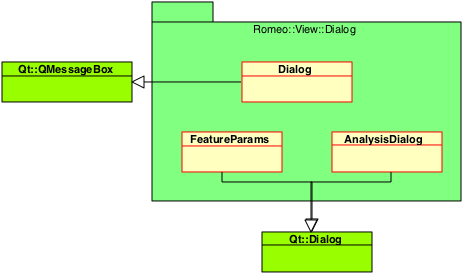
\includegraphics[width=\linewidth]{./Content/Immagini/Romeo__View__Dialog.png}
			\caption{Componente Romeo::View::Dialog}
			\label{comp_romeo::view::dialog}
		\end{figure}	
		\subsubsection{Descrizione}
		\label{descr_dialog}
		Package\glossario{} che contiene l'insieme dei \lq\lq{}dialoghi\rq\rq{} con i quali l'utente può interagire durante l'esecuzione di \project{}.
		\subsubsection{Classi contenute}

		\paragraph{\underline{FeatureParams}}
		\label{featureparams}
			\subparagraph{Descrizione:} classe che rappresenta il dialogo con il quale l'utente interagisce per selezionare la feature\g{} da aggiungere al protocol\g{}.
			\\Inoltre permette all'utente di settare i vari parametri.
			\subparagraph{Eredita da:}
				\begin{itemize}
					\item Qt::QDialog;
				\end{itemize}
			\subparagraph{Relazioni con altre classi:}
				\begin{itemize}
					\item \hyperref[]{Romeo::Controller::NewProtocolController:} relazione entrante, il controller si occupa di creare un'istanza di FeatureParams quando l'utente sceglie di aggiungere una nuova feature\g{} ad un Protocol\g{}.
				\end{itemize}
				
		\paragraph{\underline{AnalysisDialog}}
		\label{eav}
			\subparagraph{Descrizione:} questa classe rappresenta la finestra nella quale verranno mostrati i risultati intermedi di un'analisi durante la sua esecuzione. Permette inoltre di interrompere l'analisi oppure di fermare la visualizzazione dei risultati intermedi. Contiene una barra di avanzamento che si aggiorna dinamicamente all'avanzare dell'analisi, informando l'utente sullo stato della stessa.
			Viene creata ogni qualvolta l'utente seleziona la funziona di avvio analisi dalla finestra \hyperref[sav]{AnalysisView}. Emette signal\g{} verso il relativo controller, riguardo alle opzioni di visualizzazione dei risultati, oltre che per l'annullamento dell'analisi.
			\subparagraph{Eredita da:}
				\begin{itemize}
				\item Qt::QDialog.
				\end{itemize}
			\subparagraph{Relazioni con altre classi:}
				\begin{itemize}
					\item \hyperref[controller_sa]{Romeo::Controller::AnalysisController:} relazione entrante, l'AnalysisController quando richiesto si occupa della sua creazione e del suo aggiornamento;
				\end{itemize}
				
		\paragraph{\underline{Dialog}}
		\label{dia}
			\subparagraph{Descrizione:} classe che rappresenta i possibili messaggi che il sistema può inviare all'utente durante l'utilizzo di \project{}.
			\subparagraph{Eredita da:}
				\begin{itemize}
				\item Qt::QMessageBox.
				\end{itemize}


	\pagebreak

%%%%%%%%%%%%%%%%%%%%%%%%%%%%%%%%%%%%%%%%%%%%%%%	

	\subsection{Romeo::View::Component}
	\label{romeo::view::component}
		\subsubsection{Informazioni sul package}
		\label{info_component}
		\begin{figure}[!h]
			\centering
			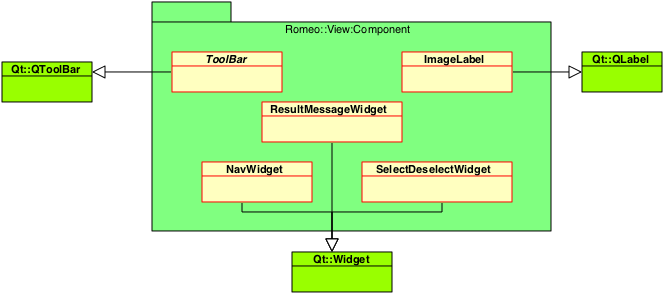
\includegraphics[width=\linewidth]{./Content/Immagini/Romeo__View__Component.png}
			\caption{Componente Romeo::View::Window}
			\label{comp_romeo::view::component}
		\end{figure}
		\subsubsection{Descrizione}
		\label{descr_component}
		Package\glossario{} contenente le classi comuni a tutte le \lq{}\lq{}view\lq{}\lq{}.
		
		\paragraph{\underline{ToolBar}}
		\label{tb}
			\subparagraph{Descrizione:} classe che rappresenta una \textit{toolbar} nella parte alta delle viste la quale permette all'utente di navigare all'interno del programma ed accedere a tutte le funzionalità.
			Viene visualizzata in tutte le viste tranne nella \textit{WelcomeView}.
			\subparagraph{Eredita ta:}
				\begin{itemize}
					\item Qt::QToolBar;
				\end{itemize}
			\subparagraph{Relazioni con altre classi:}
				\begin{itemize}
					\item \hyperref[mainview]{Romeo::View::Window::MainWindow:} relazione entrante, riferimento alla tool bar con la quale l'utente interagisce.
				\end{itemize}
			
		\paragraph{\underline{NavWidget}}
		\label{nav} 
			\subparagraph{Descrizione:} classe che rappresenta il widget costituisce la parte bassa delle view; contiene pulsanti utili, per esempio il  pulsante \emph{back}, \emph{help}, \emph{save} a seconda della view che riferisce un oggetto di questa classe.
			
			\subparagraph{Eredita da:}
				\begin{itemize}
				\item Qt::QWidget.
				\end{itemize}
	
	\paragraph{\underline{SelectDeselectWidget}}
		\label{selDel} classe che rappresenta il widget che da la possibilità all'utente di selezionare/deselezionare l'intero elenco di elementi.
		\\In questo modo si permette all'utente di velocizzare alcune operazioni, invece di dover selezionare un elemento alla volta.
		\subparagraph{Eredita da:}
			\begin{itemize}
			\item Qt::QWidget.
			\end{itemize}
			
	\paragraph{\underline{ImageLabel}}
			\label{nav} 
				\subparagraph{Descrizione:} classe che rappresenta le immagini presenti nelle viste \textit{SubjectView} e \textit{DetailedResults} con cui l'utente può interagire.
				
				\subparagraph{Eredita da:}
					\begin{itemize}
					\item Qt::QLabel.
					\end{itemize}
				\subparagraph{Relazioni con altre classi:}
					\begin{itemize}
						\item \hyperref[mainview]{Romeo::View::Window::SubjectView} 
						\item \hyperref[mainview]{Romeo::View::Window::ImageResult} 
					\end{itemize}
					
	\paragraph{\underline{ResultMessageWidget}}
				\label{nav} 
					\subparagraph{Descrizione:} classe che rappresenta dei messaggi visivi per l'utente, di successo o di errore, in tutte le viste in base alle azioni che intraprende l'utente.
					
					\subparagraph{Eredita da:}
						\begin{itemize}
						\item Qt::QWidget.
						\end{itemize}
